
\chapter{EXPERIMENTAL SETUP AND PROCEDURES}

\section{Experiment Overview}
We measured the $^{25}$Mg(d,p)$^{26}$Mg reaction  at the Research Center for Nuclear Physics (RCNP) of the Osaka University using the AVF Cyclotron, the WS course and Grand Raiden (GR) spectrometer. The layout of the facility is shown in Figure.\ref{fig:RCNP_layout}. The deuteron beam was accelerated to 56 MeV by the  K = 140 MeV Azimuthally Varying Field (AVF) cyclotron and transported to the  GR through the WS beam line. For highest resolution the beam line was dispersion matched to the GR spectrometer.

\begin{figure}[tpb]
  \begin{center}
    \centerline{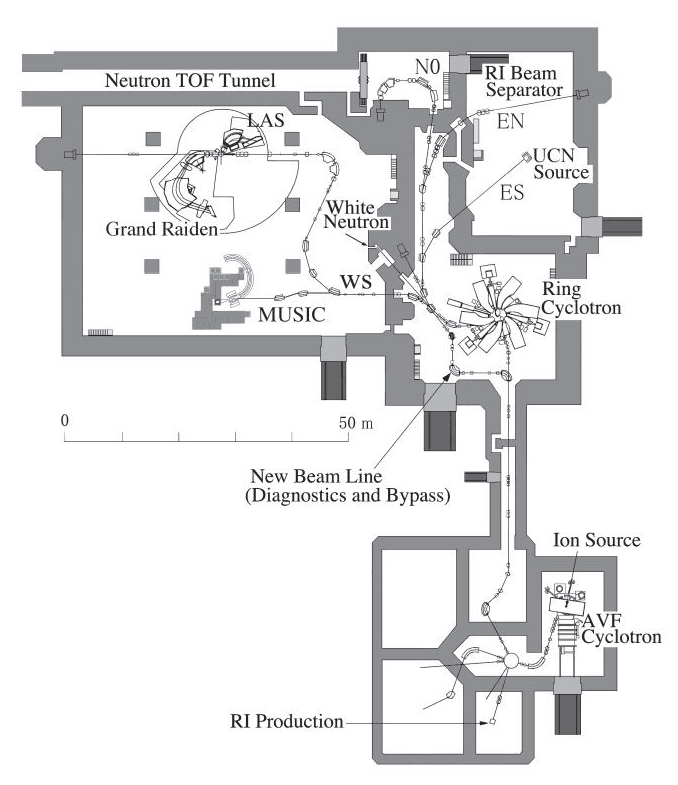
\includegraphics[scale=0.6]{graph/ch3/RCNP_layout}}
    \caption{Floor plan of the experimental facility at RCNP. The Ring Cyclotron was bypassed in this experiment.~\citep{Hatanaka2013}
    }
    \label{fig:RCNP_layout}
  \end{center}
\end{figure}
   % 

A self-supporting $^{25}$Mg target (enrichment $\approx$ 97.8$\%$) with a thickness of 1 mg/cm$^2$ was placed at the center of the scattering chamber. The total energy resolution of approximately 20 keV was  achieved, resulting from 10 keV energy loss and 4.5 keV of energy straggling of the scattering protons, as well as 1 keV of target inhomogeneity and 2.5 keV from the GR resolving power of 37000. In addition, a $^{24}$Mg target with the thickness of 1.2 mg/cm$^2$ and Mylar foils [(C$_{10}$H$_8$O$_4$)$_n$] of 6$\mu$m/(29 mm $\times$ 29 mm) were used for background measurements of reactions on carbon and oxygen.

%%%%%%
The GR spectrometer was originally placed at 0$^\circ$. The full acceptance was 20 mrad in the horizontal direction and 40 mrad in the vertical direction. The deuteron beam was dumped into the Faraday Cup inside the first dipole (D1) magnet, which is shown in Fig \ref{fig:GR_FC}. This Faraday Cup was also used for monitoring the beam current. For scattering angles in the range of $2^\circ \textendash 6 ^\circ$ the Faraday cup Q1-FC downstream of the quadrupole Q1 was used. For larger angles, the Faraday cup in the scattering chamber was employed.
In order to achieve best possible spatial and angular resolution, full dispersion matching\citep{Wakasa200279} including the over-focus mode \citep{FUJITA200217} were applied. Outgoing protons were momentum analyzed and focused at the focal plane where the focal plane detector system was placed. The focal plane detector system consisted of two multi-wire drift chambers (MWDCs)  and two plastic scintillators. Particles were then traced back with  the MWDCs allowing the reconstruction of particle trajectory. The protons were identified with the scintillators by the timing and energy loss differences. The scintillators also produced  the start and stop triggers for the MWDCs.


%Protons scattered by the target placed in the target chamber were analyzed by the GR %spectrometer and detected by the Focal Plane Detectors at the end of the beam line.



\section{The Grand Raiden Spectrometer}
The Grand Raiden (GR) spectrometer was designed for high resolution measurements. It consists of three dipoles (D1, D2 and DSR) magnets, two quadrupole  (Q1 and Q2) magnets, a sextupole  (SX)  magnet and a multipole  (MP) magnet (See Fig.~\ref{fig:GR_layout}). The design parameters of the specification and ion-optical properties are listed in Table.~\ref{tb:GR}. Its large magnetic rigidity of B$\rho=$5.4 T$\cdot$m  and high resolving power of $p/\Delta p=\dfrac{D_x}{M_x \Delta x_0}=37000$ (where $\Delta x_0$ = 1 mm for a monochromatic beam spot size, $M_x$ and $D_x$ refer to the magnification and the dispersion of the spectrometer, respectively) make it stand out for high resolution measurement.
The Q1 magnet is placed close to the scattering chamber in order to achieve large vertical angle acceptance.
The second-order ion-optical aberrations are in part minimized by the SX magnet. The MP magnet generating the quadrupole, sextupole, octupole and decapole is installed between the D1 and D2 magnet to further correct higher-order aberrations. The DSR magnet is an auxiliary magnet for measuring the spin-rotation parameters and was not used in the present experiment. The GR spectrometer is designed in such way that particles with different magnet rigidities are transported to different horizontal positions in the focal plane.

\begin{figure}[tpb]
  \begin{center}
    \centerline{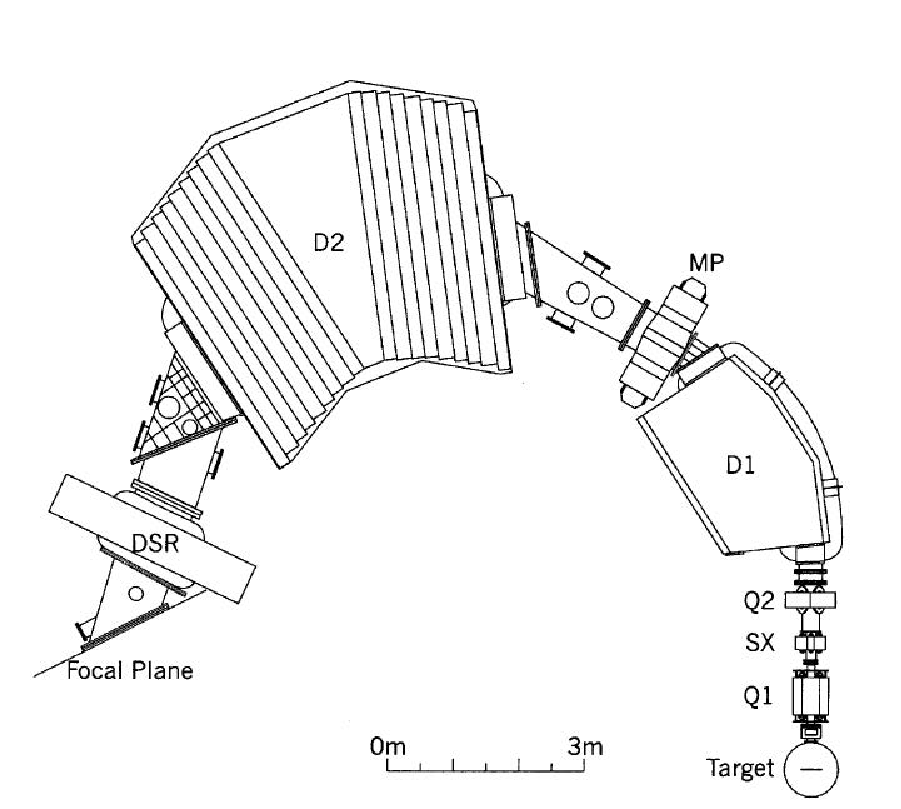
\includegraphics[scale=0.7]{graph/ch3/GR_layout}}
    \caption{The schematic layout of the Grand Raiden (GR) Spectrometer. ~\citep{Wakasa200279} }
    \label{fig:GR_layout}
  \end{center}
\end{figure}


\begin{table}[tpb]
  \setlength{\capwidth}{0.7\textwidth}
  \begin{center}
    \caption{DESIGN VALUES FOR THE GRAND RAIDEN SPECTROMETER ~\citep{Fujiwara1999484} }
    \label{tb:GR}
    \begin{tabular}{lr} \toprule
      \hline
      Mean orbit radius                         &           3 m \\
      Total deflection angle                    &           162$^{\circ}$\\
      Angular range                             &           0$^{\circ}$ to 90$^{\circ}$\\
      Focal plan length                         &           150 cm\\
      Tilting angle of focal plane              &           45.0$^{\circ}$\\
      Maximum field strength of dipoles (D$_1$, D$_2$)    &       1.8 T\\
      Vertical magnification (M$_y$)            &           5.98\\
      Horizontal magnification (M$_x$)          &           -0.417\\
      Momentum dispersion (D$_x$)               &           15.45 m\\
      Momentum range                            &           5\%\\
      Momentum resolution (p/$\Delta$p)         &           37000\\
      Horizontal acceptance angle               &           $\pm$ 20 mrad\\
      Vertical acceptance angle                 &           $\pm$ 40 mrad\\
      Solid angle                               &           3.2 msr \\\bottomrule
    \end{tabular}
  \end{center}
\end{table}



\section{Dispersion Matching}
The high resolving power of the  spectrometer gives an optimum energy resolution of about 2.5 keV for  56 MeV deuterons  for a monochromatic image size on target of $\Delta  x = 1$ mm ($\Delta K=(1.70\cdot \Delta p/p)K = 2.5$ keV). However, the momentum spread of the incident beam produced by the cyclotron usually makes the spectral resolution worse in the achromatic beam transportation. To achieve the high resolution measurement, the dispersion of the beam line and the dispersion of a spectrometer has to be  matched.
The dispersion matching method can be explained by using matrices for ion optics in the TRANSPORT notations in the phase space. A particle in the system can be described by coordinates $\boldsymbol{x}=(x, \theta, \delta)$, where the $x$, $\theta$ and $\delta$ are the horizontal displacement, angle and fraction of the momentum deviation defined by $p/\Delta p$ respectively,  and they are defined as differences from the central trajectory.
Assume particles pass through the exit point of the accelerator with the coordinates $\boldsymbol{x_0}=(x_0, \theta_0, \delta_0)$ and end up with the coordinates $\boldsymbol{x_1} =(x_1, \theta_1, \delta_1)$ at the target position after transport through the beam line system  described by the matrix $\textbf{B}=\{b_{\mu \nu}\}$, where the matrix elements represent $x$, $\theta$, $\delta$ with 1, 2 and 6, respectively. $\delta_0=\delta_1$, $b_{61}=b_{62}=0$ and $b_{66}=1$ as the energy does not change in the magnetic field.
Particles are then scattered in the target position with $\boldsymbol{x_2}=(x_2, \theta_2, \delta_2)$ by the target matrix $\textbf{T}$ and reach the focal plane with $\boldsymbol{x}=(x, \theta, \delta)$ transported by the spectrometer matrix $\textbf{S}=\{s_{\mu \nu}\}$. By combining $\textbf{B}$, $\textbf{T}$ and $\textbf{S}$, the transformations at the focal plane position are given by
\begin{equation}
    \label{eq:x_fp}
    \begin{aligned}
     x_{fp} & =  x_0(s_{11} b_{11} T + s_{12} b_{12})               \\
            & + \theta_0(s_{11} b_{12} T + s_{12} b_{22})          \\
            & + \delta_0(s_{11} b_{16} T + s_{12} b_{26} + s_{16} C)  \\
            & + \Theta(s_{12} + s_{16} K)                           \\
    \end{aligned}
\end{equation}
\begin{equation}
    \label{eq:theta_fp}
    \begin{aligned}
     \theta_{fp} &= x_0(s_{21} b_{11} T + s_{22} b_{21})        \\
                 &+ \theta_0(s_{21}b_{12}T + s_{22} b_{22})     \\
                 &+ \delta_0(s_{21}b_{16}T + s_{22}b_{26} + s_{26}C) \\
                 &+ \Theta(s_{22} + s_{26}K)                    \\
    \end{aligned}
\end{equation}
where $T$, $C$, $K$ are the target function, the dispersion-matching factor and  kinematic factor,  respectively,  and defined as
\begin{equation}
    \label{eq:TKC}
    \begin{aligned}
     T & = \frac{\cos(\alpha - \phi_T)}{\cos \phi_T}                        \\
     C & = \frac{p_{in}}{p_{out}} \cdot \frac{\partial p_{out}}{\partial p_{in}} \\
     K & = \frac{1}{p_{out}} \cdot   \frac{\partial p_{out}}{\partial \alpha}  \\
    \end{aligned}
\end{equation}

\begin{figure}[tpb]
  \begin{center}
    \centerline{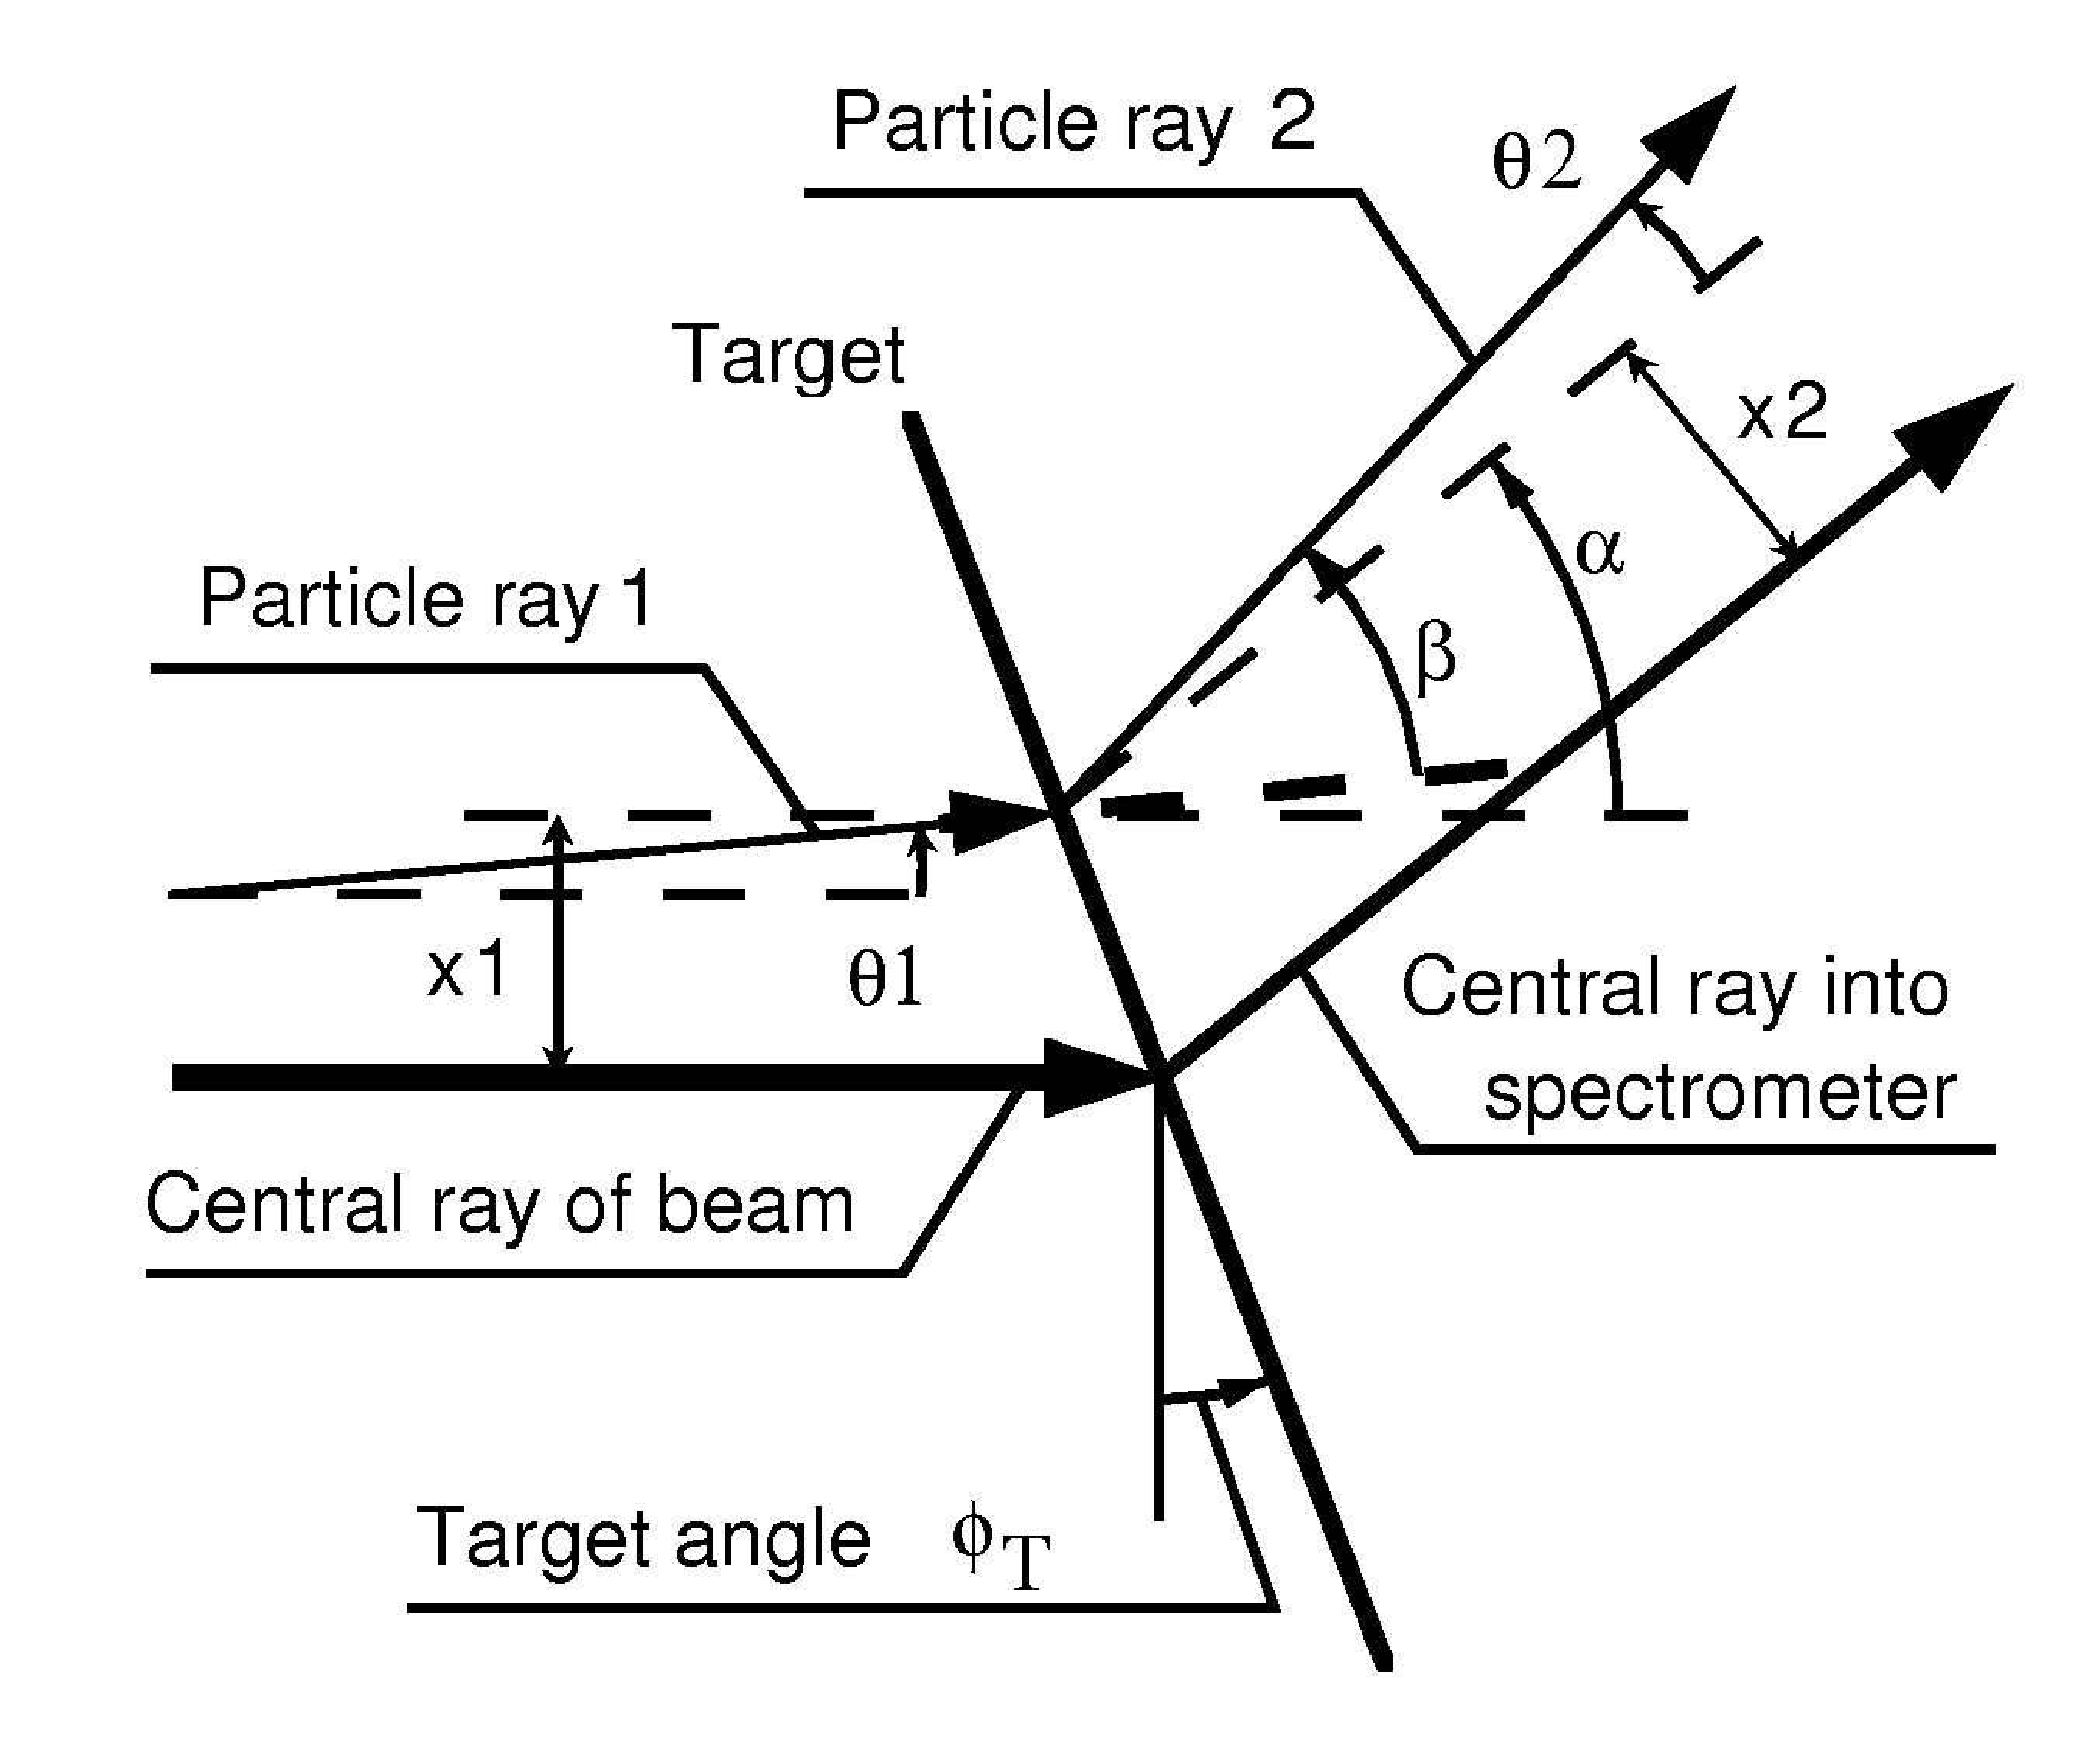
\includegraphics[scale=0.18]{graph/ch3/kinectics}}
    \caption{Schematic representation of the scattering of one particle with coordinates ($x_1$, $\theta_1$ )
relative to the central ray of the beam. The ($x_2$, $\theta_2$) are coordinates of outgoing particles and $\alpha$ is the
scattering angle of the central ray.}
    \label{fig:kinectics}
  \end{center}
\end{figure}

In the target function $T$, $\alpha$ is the reaction angle in the laboratory frame and $\phi_T$ is the tilting angle of the target. In the dispersion-matching factor $C$, $p_{out}$ is the momentum of the outgoing particle at the target and $p_{in}$ is the momentum of the incident particle at the target position. There are several special cases can simplify the calculation. For instance, for an elastic scattering, $C=1$ and at 0$^\circ$, the kinematic factor $K=0$.
The geometry of the kinematics is illustrated in Fig. ~\ref{fig:kinectics}, where $\theta_1$ is the angle between the incident particle  and the central ray of the beam and $\theta_2$ is the angle between the outgoing particle and the central ray into the spectrometer. The true scattering angle is thus given by
\begin{equation}
    \label{eq:beta}
    \begin{aligned}
    \beta=\alpha+(\theta_2-\theta_1)
    \end{aligned}
\end{equation}
The momentum at the focal plane is then given as
\begin{equation}
    \label{eq:sigma_fp}
    \begin{aligned}
    \delta_{fp} = \theta_2 = K \Theta + C\delta_0
    \end{aligned}
\end{equation}
where $\Theta=\theta_1-\theta_2$ is the relative scattering angle.


The best possible spectral resolution can be achieved by minimizing the image size of $x_{fp}$ as well as realizing the angular dispersion matching. As a result, the coefficients of  $\theta_0$, $\sigma_0$ and $\Theta$ in  Eq.~\ref{eq:x_fp}  should be eliminated and the coefficient of $\delta_0$ in Eq.~\ref{eq:theta_fp} should be minimized. The $\delta_0$ dependence of $\theta_{fp}$ in Eq.~\ref{eq:theta_fp} is large since a large dispersion $b_{16}$ of the beam line is required for the lateral dispersion matching.

The minimization of the coefficient of $\Theta$ in Eq.~\ref{eq:x_fp} gives
 \begin{equation}
    \label{eq:s12}
    \begin{aligned}
        s_{12} = -s_{16}K
    \end{aligned}
\end{equation}
which is called the kinematic correction.

The minimization of the $\theta_0$ dependence in Eq.~\ref{eq:x_fp} results in
 \begin{equation}
    \label{eq:b_12}
    \begin{aligned}
        b12=-\frac{s_{12}}{s_{11}}\frac{b_{22}}{T}
    \end{aligned}
\end{equation}
which is known as the focusing matching.

To realized the so-called the dispersion matching, by minimizing the coefficients in  $\sigma_0$ in  Eq.~\ref{eq:x_fp} both lateral dispersion matching and angular dispersion matching can be  achieved by setting the matrix elements of the beam line as:
 \begin{equation}
    \label{eq:b16}
    \begin{aligned}
        b_{16} = -\frac{s_{16}}{s_{11}}(1 + s_{11}s_{26}K - s_{21}s_{16}K)\frac{C}{T}
    \end{aligned}
\end{equation}
and
 \begin{equation}
    \label{eq:b26}
    \begin{aligned}
        b_{26} = (s_{21}s_{16} - s_{11}s_{26})C
    \end{aligned}
\end{equation}
Here the relationship $s_{11}s_{22}-s_{12}s_{21}=1$ is used to make the expression simpler. The matching conditions given by Eq.~\ref{eq:b16} and Eq.~\ref{eq:b26} are the so-called the lateral dispersion matching and the angular dispersion matching, respectively.

The resolving power of the matched system is given by
 \begin{equation}
    \label{eq:R}
    \begin{aligned}
        R=(1/2x_0)(s_{16}/M_{ov})
    \end{aligned}
\end{equation}
where $M_{ov}=(s_{11}b_{11}T+s_{12}b_{12})$ refers to as an overall magnification and has the form
 \begin{equation}
    \label{eq:M}
    \begin{aligned}
        M=(s_{11}b_{11}T-s_{16}b_{12}K)
    \end{aligned}
\end{equation}
if the matching conditions are satisfied.


The concept of dispersion matching conditions is shown in Fig.~\ref{fig:dispersion}. Only trajectories of central rays scattered at 0$^{\circ}$ are shown in these figures. In the left panel (a), three trajectories with different momenta $\sigma_0=0$, $\pm\Delta p/p$ are shown for a beam with the achromatic focus at the target position ($b_{16}=b_{26}=0$). Particles with different $\delta_0$ are dispersed by the spectrometer and the resolution focused in the focal plane are limited by the beam momentum spread.
The middle panel (b) shows beam trajectories when the lateral dispersion-matching is realized ($b_{16}$ matched, $b_{26}=0$).
Particles with different momenta $\delta_0$ are focused at different lateral positions on the target and this dispersion is compensated by the dispersion of the spectrometer. In such way the spectral resolution is no longer limited by the momentum spread of the beam.
However, under this condition, rays with different $\delta_0$ may cross the focal plane with different angles $\theta_{fp}$, which gives rise to an ambiguity in determining the scattering angles at the target. This can be eliminated when both lateral and angular dispersion-matching have been realized simultaneously, which is shown in the right panel (c). By adjusting the dispersion of the positions and incident angles for beam rays appropriately, the positions and angles of particles measured at the focal plane ($x_{fp}$, $\theta_{fp}$) do not depend on the beam dispersion at the target and the measured angle in the focal plane corresponds to a unique scattering angle.




\begin{figure}[tpb]
  \begin{center}
    \centerline{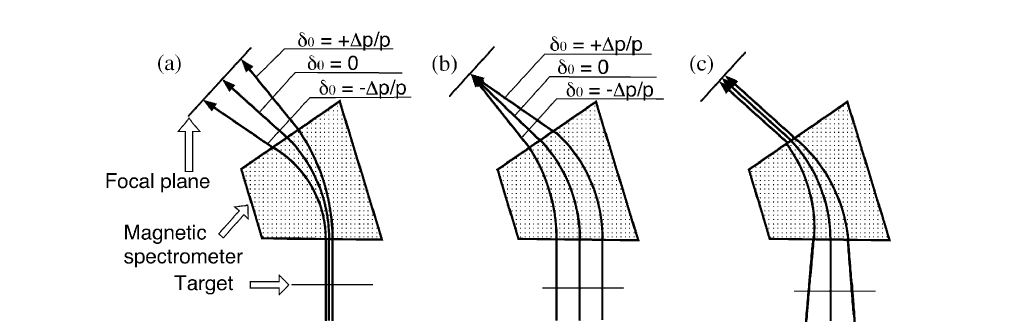
\includegraphics[scale=0.7]{graph/ch3/dispersion}}
    \caption{Schematic ion trajectories under different matching conditions of a beam line and a magnetic spectrometer.(a)When achromatic mode is achieved; (b)when lateral dispersion matching is realized; (c)when both lateral and angular dispersion matching are realized. The rays with the different momenta are shown.~\citep{FUJITA200217}}
    \label{fig:dispersion}
  \end{center}
\end{figure}


\section{0$^{\circ}$ Measurement and the Over-focus Mode}
In order to determine the angular distribution, an angular measurement is needed with a good resolution. Near and including 0$^{\circ}$, high resolution measurements of both horizontal and vertical angle components  are equally important such that the scattering angle can be precisely determined. However, since GR spectrometer is a horizontal-bending high-resolution spectrometer, the vertical angle magnification is small ($\approx$ 0.17)  so that the vertical focusing quadrupole magnet is placed as close to the target as possible in order to realize a large vertical acceptance.
Under this condition, it is impossible to achieve a vertical resolution at the target better than 12 mrad. Therefore, the vertical angle resolution cannot be determined as good as the horizontal angle resolution in the normal point-to-point focus mode.

In order to improve the vertical angular resolution, the ion-optical mode called off-focus mode has been developed at RCNP.  The ion-optical properties of the spectrometer in the vertical direction were considered in the transfer matrix up to the second order:
 \begin{equation}
    \label{eq:y_fp}
    \begin{aligned}
        y_{fp} &= (y|y)y_{tgt}+(y|\phi)\phi_{tgt} + (y|yx)y_{tgt}x_{tgt} \\
               &+ (y|\theta)y_{tgt}\theta_{tgt} + (y|y\delta)y_{tgt}\delta \\
               &+ (y|\phi x)\phi_{tgt} x_{tgt} + (y|\phi \theta) \phi_{tgt} \theta_{tgt} \\
               &+ (y|\phi \theta) \phi_{tgt} \delta           \\
               &+higher \ order \ terms
    \end{aligned}
\end{equation}
where $y_{tgt}$ and $\phi_{tgt}$ are the vertical position and the outgoing angle of a particle at the target and $x_{tgt}$ and $\theta_{tgt}$ are the horizontal position and angle, respectively. $(y|y)$, $(y|\phi)$ etc. are matrix elements of the spectrometer  that transports coordinates from the target to the focal plane coordinates.  $\delta$ is the fractional momentum spread of the incoming beam at the target.


In Fig.~\ref{fig:off_focus} the vertical trajectories for three different focus modes are depicted. In the normal focus mode of GR spectrometer shown in the top panel (a), the term $(y|\phi)$  from Eq.~\ref{eq:y_fp} is set to  zero for the central ray (R = 300 cm). By increasing the strength of the Q1 magnet of GR spectrometer such that $(y|\phi)>0$, particles with different vertical outgoing angles from the target, $\phi_{tgt}$, will be transported to different vertical positions $y_{fp}$ in the focal plane. This mode is called over-focus mode and the vertical trajectories are shown in the middle panel (b). Similarly, the bottom panel (c) shows trajectories of the transport in the under-focus mode where the strength of the Q1 magnet is decreased and $(y|\phi)<0$. Therefore, it is possible to determine  $\phi_{tgt}$ values from the measured value of $y_{fp}$ in the off-focus modes.
\begin{figure}[tpb]
  \begin{center}
    \centerline{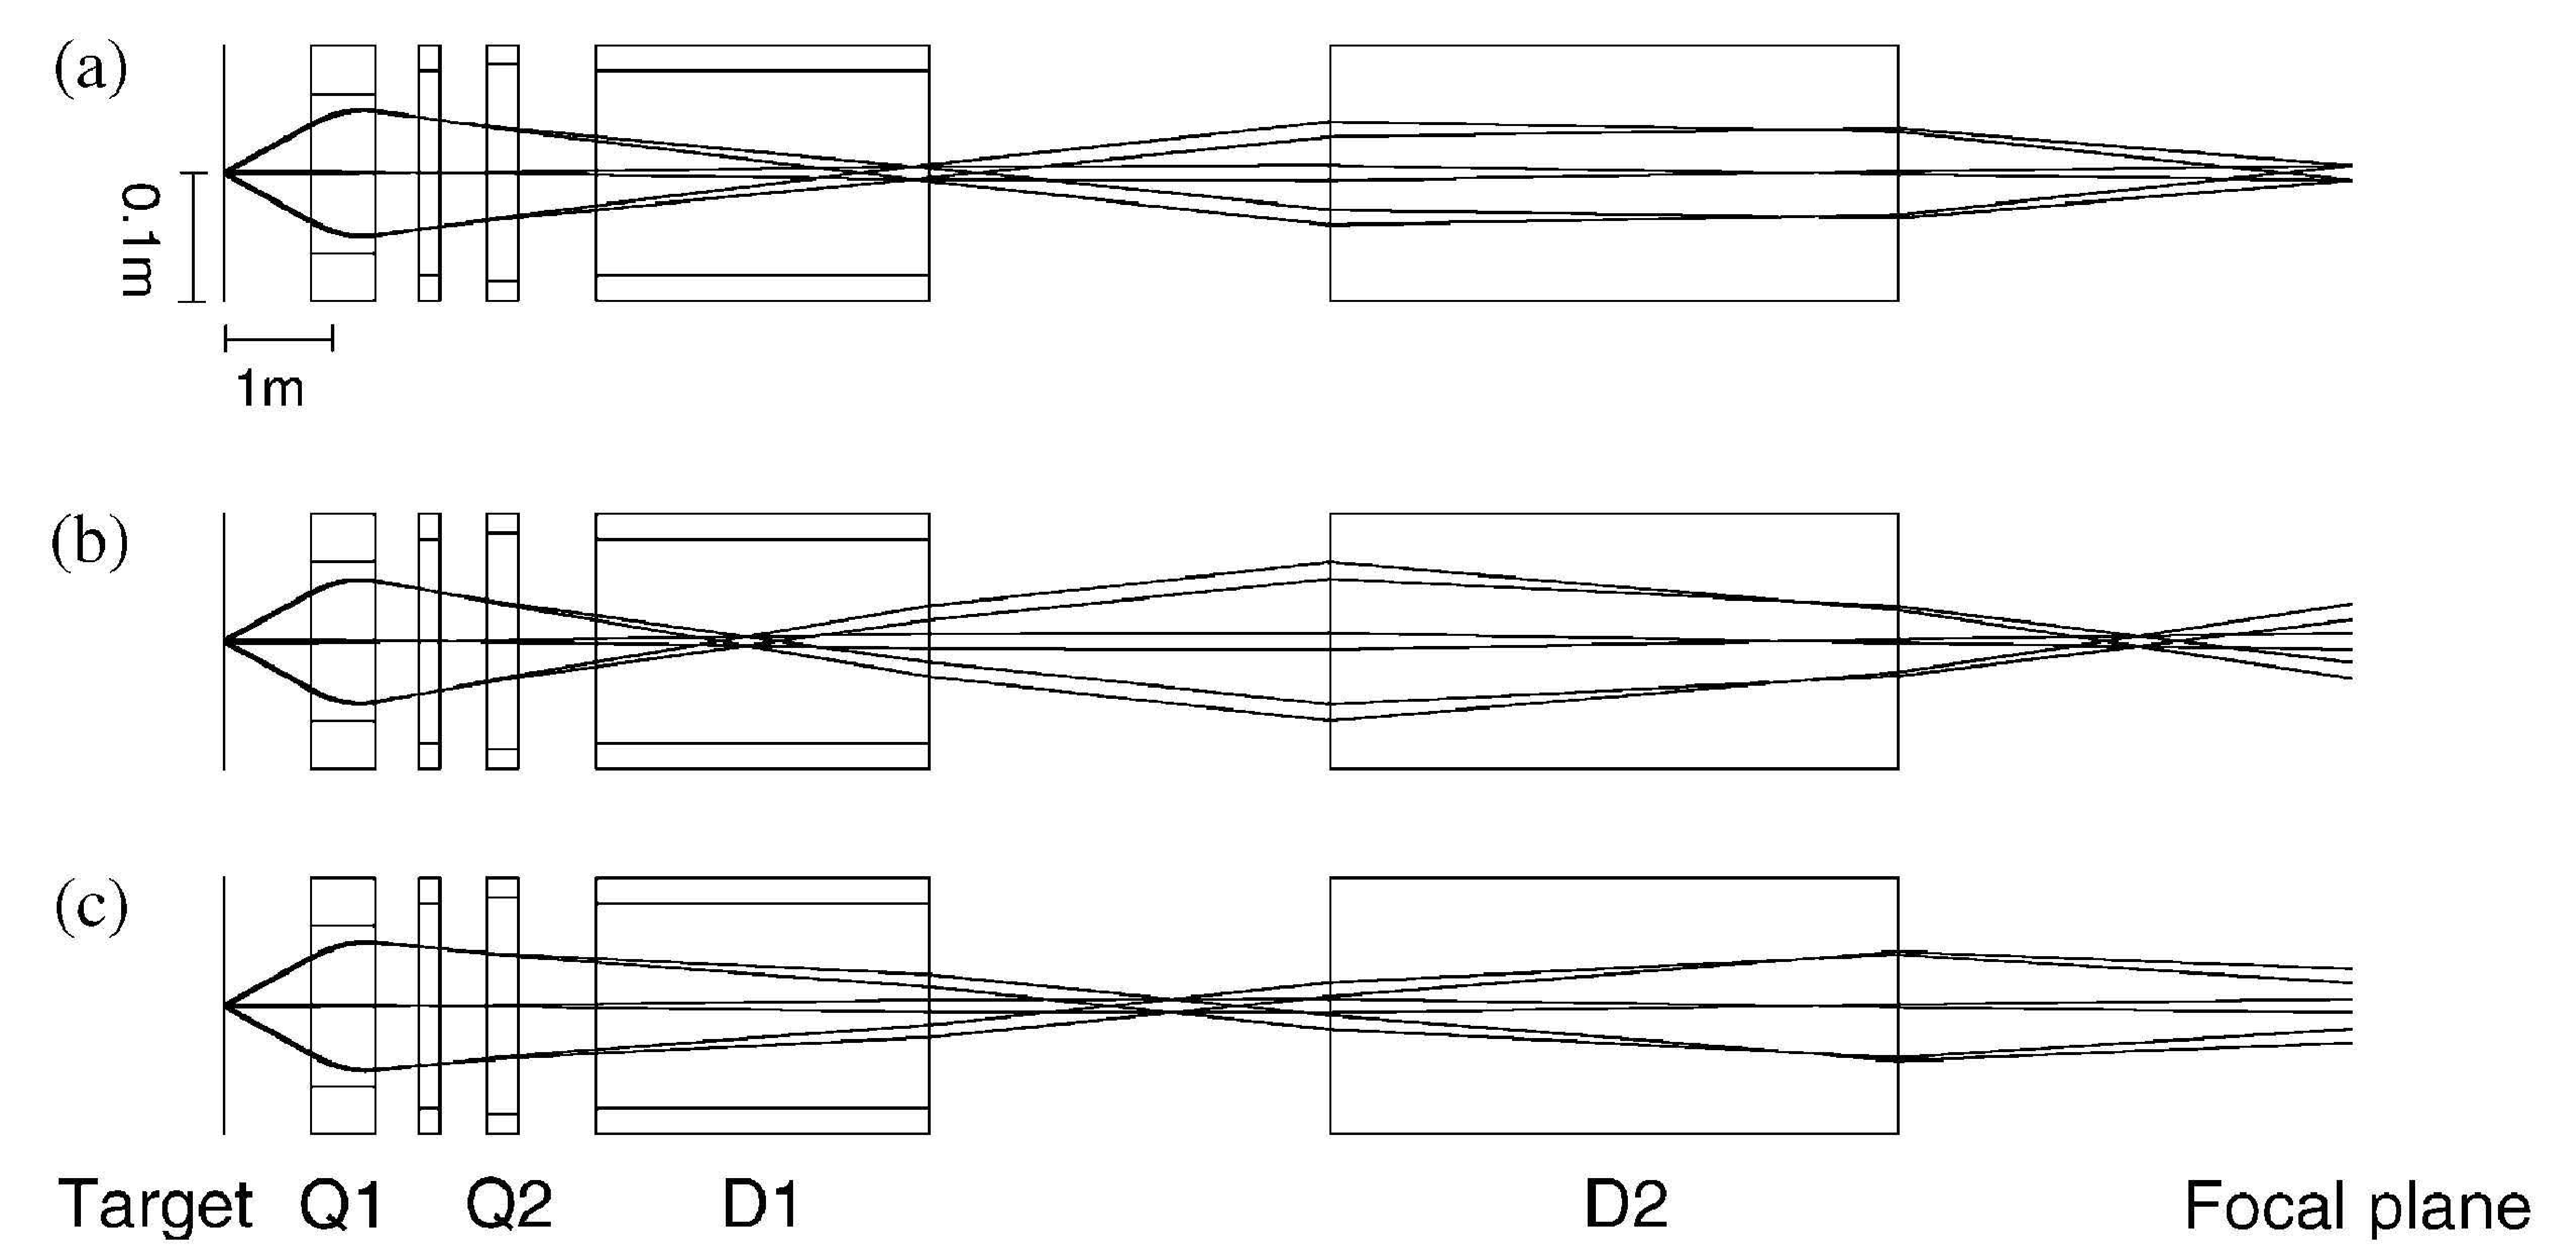
\includegraphics[scale=0.15]{graph/ch3/focus_mode}}
    \caption{Envelope of analyzed particles in Grand Raiden for vertical position with $\phi_{tgt}=0$, $\pm$46 mrad and $y_{tgt}=\pm$1. (a) Normal focus mode. (b) Over focus mode. (c) Under focus mode.~\citep{FUJITA200155}}
    \label{fig:off_focus}
  \end{center}
\end{figure}
In order to calibrate vertical components of scattering angle $\phi_{tgt}$ in the off-focus mode accurately, the ambiguities from the angle determination should be small. The largest ambiguity comes from the vertical beam spot size  $\Delta y_{tgt}$ due to the large  vertical magnification $(y|y)$ of about 6. Typically, $\Delta y_{tgt}$ is $0.5\textendash 1$ mm, so the $(y|y)\Delta y_{tgt}$ term can bring about $3\textendash6$ mm uncertainty in the vertical focal plane. Such effect can be minimized by  increasing the absolute value of the $(y|\phi)$ term which is adjusted by the strength of the quadrupole magnet Q1.

The experiment was performed in the over-focus mode by increasing the Q1 strength by 8\% as compared with the  normal point-to-point focus. In order to  reconstruct the coordinates at the target position from the measured coordinates at the focal plane, a multi-hole aperture (sieve-slit) was used for the angle calibration.


\section{Focal Plane Detectors}
In the focal plane of the GR spectrometer, two 2-dimensional multi-wire drift chambers (MWDCs) were used in order to measure the positions and angles of the outgoing particles. A set of 3 mm and 10 mm thick $\Delta$E plastic scintillator detectors followed by MWDCs was used to provide energy loss and timing information for particle identification. To increase the energy loss in the plastic sintillators, an aluminum degrader (10 mm thick) was placed between the MWDCs and the plastic sintillators. The layout of the focal plane detector system is illustrated in  Fig.~\ref{fig:PSs}. Under this setting the protons produced by the (d,p) reaction are stopped before they reach the last  plastic scintillator.

\begin{figure}[tpb]
  \begin{center}
    \centerline{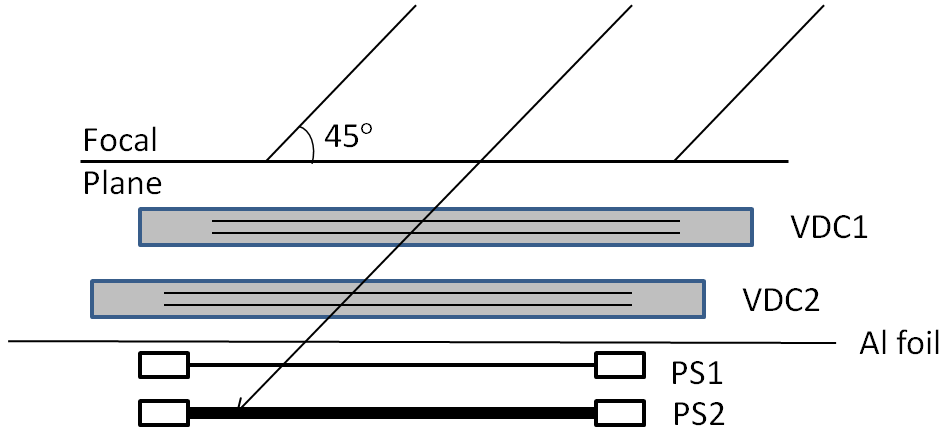
\includegraphics[scale=0.6]{graph/ch3/PSs_new}}
    \caption{Schematic layout of the focal plane detector system. PS1 is 3mm and PS2 is 10mm. An Al degrader is placed in front of the PS1.}
    \label{fig:PSs}
  \end{center}
\end{figure}

The MWDC is also known as the vertical drift chamber (VDC) as  ionized electrons drift perpendicularly to the anode plane. The specifications of the MWDC are listed in Table.~\ref{tb:MWDC}. Each 2-dimensional MWDC consists of two anode-wire planes (X and U) sandwiched between three cathode planes. Anode planes consist of sense wires and potential wires as is depicted in  Fig.~\ref{fig:MWDCs}. The spacing of sense wires is 6 mm for the X-plane and 4 mm for the U-plane, respectively. The potential wires are designed in such way to produce uniform electric field between the cathode plane and the anode plane, supplying the high voltage of -350 V and -500 V in the X-plane and U-plane, respectively. Thus electrons generated by charged particles during the ionization of the detector gas can only produce avalanche near the sense wires. A charged particle trajectory are determined by  measuring the drift-time  of the electrons from four wires, as shown in Fig.~\ref{fig:MWDCs}. For a proper trajectory determination, at least three wire events are  needed to for the drift time measurement per plane. The gas used in the MWDC is a mixture of argon (71.4\%), iso-butane (28.6\%) and iso-propyl-alcohol. The iso-propyl-alcohol was mixed into argon gas with vapor pressure ar 2$^{\circ}$ in order to reduce the deterioration of the gas due to  the aging effect like the polymerization of the gas on the wire surface\citep{Adachi_thesis}\citep{yosoi_thesis}.

\begin{table}[tpb]
  \setlength{\capwidth}{0.7\textwidth}
  \begin{center}
    \caption{SPECIFICATIONS OF MWDCs FOR THE GRAND RAIDEN SPECTROMETER\citep{yosoi_thesis}.}
    \label{tb:MWDC}
    \begin{tabular}{ll} \toprule
      \hline
      Wire configuration                        &           X (0$^{\circ}$ from vertical), U(48.2$^{\circ}$ from vertical) \\
      Active area                               &           1150 mm $\times$ 120 mm\\
      Number of sense wires                     &           192 (X), 208 (U)\\
      Cathode-anode gap                         &           10 mm       \\
      Anode-wire spacing                        &           2 mm\\
      Sense-wire spacing                        &           6 mm (X), 4 mm (U)\\
      Sense-wire thickness                      &           20 $\mu$ m gold-plated tungsten\\
      Potential-wire thickness                  &           50 $\mu$ m gold-plated beryllium-copper\\
      Cathode plane                             &           10 $\mu$ m carbon-aramid foil\\
      Gas mixture                               &           Argon (71.4\%), Iso-butane (28.6\%), \\
                                                &           Iso-propyl-alcohol (trace amount)\\
      Entrance and exit windows                 &           12.5 $\mu$ m aramid foil\\
      Distance between MWDCs                    &           250 mm\\
      \bottomrule
    \end{tabular}
  \end{center}
\end{table}

%\begin{figure}[tpb]
 % \begin{center}
 %   \centerline{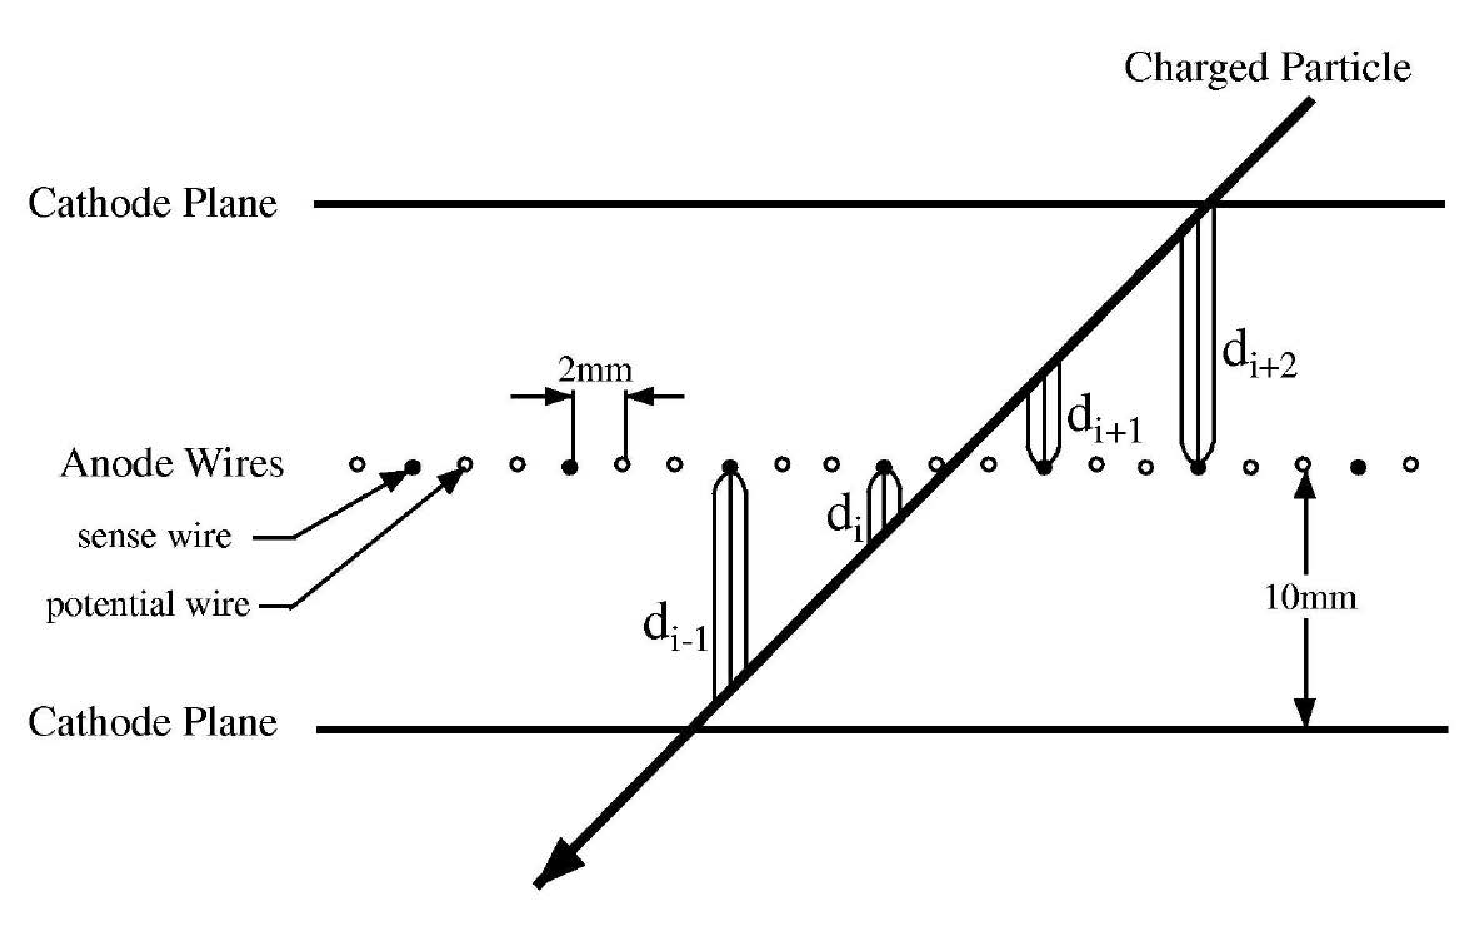
\includegraphics[scale=0.5]{graph/ch3/MWDCs}}
 %   \caption{The schematic structure of an X-plane of the MWDC. A typical track of an charged particle is shown. ~\citep{yosoi_thesis}}
 %   \label{fig:MWDCs.}
 % \end{center}
%\end{figure}

\begin{figure}[tpb]
  \begin{center}
    \centerline{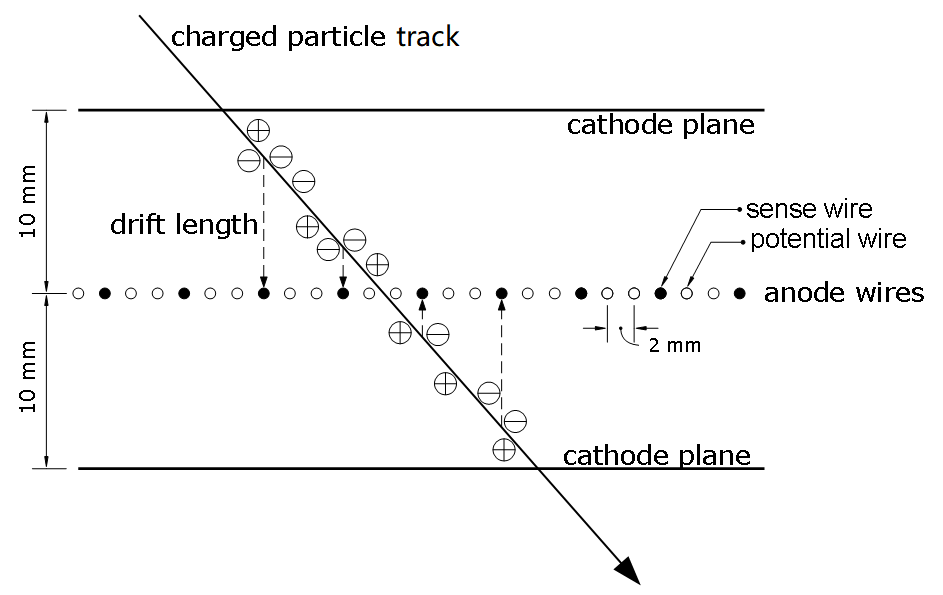
\includegraphics[scale=0.6]{graph/ch4/MWDCs_1}}
    \caption{X-plane configuration of the MWDC. A sample of the charged particle track is shown together with the cathode planes and anode wires.}
    \label{fig:MWDCs}
  \end{center}
\end{figure}

Particles that pass through the MWDCs are detected in two plastic scintillator detectors.
Each scintillator had two photomultipliers (PMs) attached on the left and right side  and were held a voltage of 1800 V and 1450 V for the 3 mm plastic scintillator and 10 mm plastic scintillator, respectively.  The fluorescence is proportional to $\Delta$E of particles, as well as the timing information were produced and collected as events  for particle identification.


\section{Faraday Cup Settings for the (d,p) Reaction}
In addition to the 0$^{\circ}$ data,  measurements were also preformed in the angular range from 5$^{\circ}$ to 40$^{\circ}$ in 5$^{\circ}$ steps. These angular distributions serve several purposes:

1. The measurement of the angular distribution will help to determine the orbital momentum of the transferred neutron.

2. Measurements at different angles allow the identification of lines due to contaminants with different masses owing to their different kinematic shift.

3. Unavoidable light-mass impurities in the target may obscure a peak at one angle but clear this peak at a different angle, allowing its identification.

The Faraday cup setting for 0$^{\circ}$ measurement is shown in Fig.~\ref{fig:GR_FC}. Owing to the differences in magnet rigidities of the deuteron beam and the proton beam from the reaction (ratios in the range of 1.324  to 1.422), the D1 Faraday cup was installed inside the D1 dipole of GR such that deuterons were bent into the Faraday cup while protons were tuned to the focal plane. Since the dispersion in the focal plane is about 15.5m, for a deuteron beam of 56 MeV this allows to measure an excitation range of about 5 MeV and covers the range of interest  about $E_x=$ 9 MeV to 14 MeV with one field setting. At 5$^{\circ}$  the Faraday cup Q1-FC downstream of the quadrupole Q1 was used. For larger angles the Faraday cup inside the scattering chamber was applied.

Nevertheless,  during the experiment there was still a huge deuteron background at 0$^{\circ}$, which was high enough to limit the measurement. This  can be reduced by changing the angle of GR spectrometer to 0.5$^{\circ}$ while still covering the 0$^{\circ}$ measurement. Even though there might still exist  small deuteron background after changing the angle, the remaining background can be removed by using information from the time of flight of the particles.

In this experiment, beam intensities up to 6 nA were used for 0.5$^{\circ}$ and up to 100 nA for higher angle measurements. The live time of the system varied between 93\% and 96\% during the experiment. Three magnet field settings were deployed to cover the whole excitation energy region of interest with sufficient overlap between the different spectra.

The energy calibration was preformed using the $^{25}$Mg(d,p)$^{26}$Mg reaction. The energies of excited states in $^{26}$Mg up to 12 MeV are well known. However, above 7 MeV the level density becomes sufficiently large that it becomes impractical to use these higher-lying states for the calibration. Therefore, protons from lower-lying states were used to calibrate the full focal plane by changing the magnetic settings with sufficient overlap between the different spectra. Three magnetic fields were established in this experiment, which allows us to determine the relatively small but not negligible quadratic term over the full focal plane.  The absolute excitation energy calibration has been  established using the locations of the peaks of the low-lying states in the target nuclei with well-known excitation energies.


\begin{figure}[tpb]
  \begin{center}
    \centerline{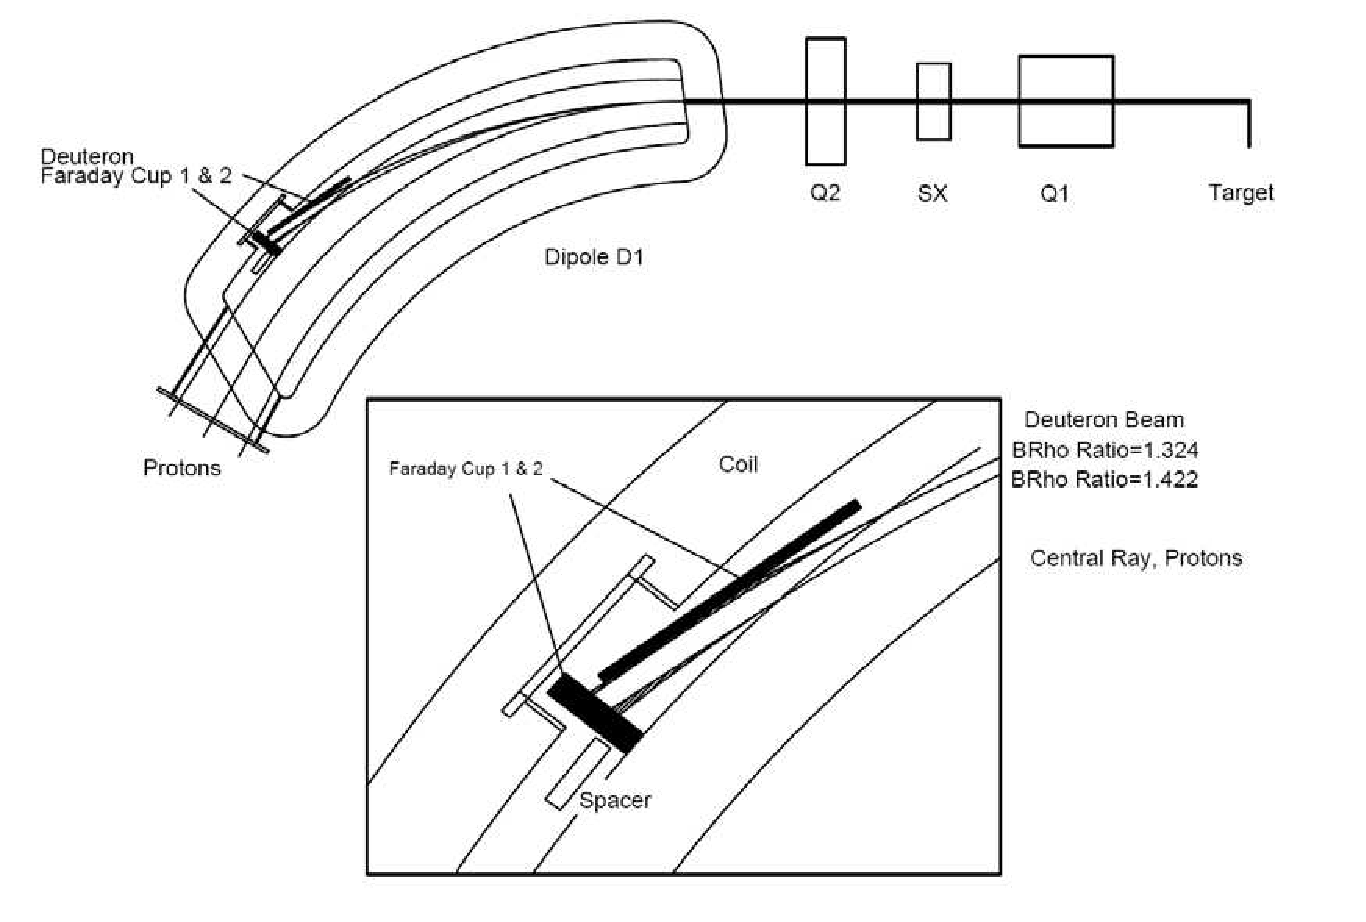
\includegraphics[scale=0.6]{graph/ch3/FC}}
    \caption{The Faraday Cups inside dipole D1 for 0$^\circ$ mode.}
    \label{fig:GR_FC}
  \end{center}
\end{figure}


% % uncomment the following lines,
% if using chapter-wise bibliography
%
 % \bibliographystyle{ndnatbib}
 % \bibliography{reference}
